% Appendix Template

\appendixpagenumbering % Restart numbering for each appendix

\chapter{AppKey Server: REST API Documentation} % Main appendix title
\label{AppendixRestApiDoc} 

This document contain all the routes available on the AppKeyServer. The \cref{figapdx-database_model} illustrate the database model used by the server.

\begin{figure}[ht!]
    \centering
    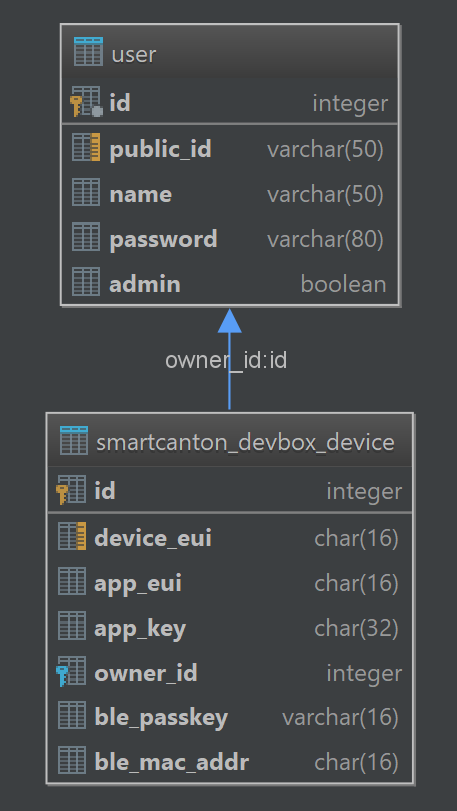
\includegraphics[width=0.4\textwidth]{Figures/Appendixes/database_model.PNG}
    \caption{Database model}
    \label{figapdx-database_model}
\end{figure}

This documentation is also provided on the root path of the server : 


\begin{tcolorbox}[top=-3mm, bottom=-3mm, left=0mm, right=0mm, enhanced, breakable, colback=LightGray, colframe=DarkGray, colbacktitle=DarkGray]
\begin{minted}[bgcolor=LightGray,fontsize=\footnotesize,breaklines]{bash}
$ curl -X GET https://127.0.0.1:5000/
\end{minted}
\end{tcolorbox}

\clearpage
%%%%%%%%%%%%%%%%%%%%%%%%%%%%%%%%%%%%%%%%%%%%%%%%%%%%%%%%%%%
\section{Authentification}
%%%%%%%%%%%%%%%%%%%%%%%%%%%%%%%%%%%%%%%%%%%%%%%%%%%%%%%%%%%

\underline{Command rights} : Anyone can request a JWT token. The only requirement it that the user/password combinaison on the POST body is correct.\\

\textbf{Curl command for a JWT authentification :}

\begin{tcolorbox}[top=-3mm, bottom=-3mm, left=0mm, right=0mm, enhanced, breakable, colback=LightGray, colframe=DarkGray, colbacktitle=DarkGray]
\begin{minted}[bgcolor=LightGray,fontsize=\footnotesize,breaklines]{bash}
$ curl -X POST \
  http://127.0.0.1:5000/auth \
  -H 'cache-control: no-cache' \
  -H 'content-type: application/json' \
  -d '{
    "username": "<YOUR_USERNAME",
    "password": "<YOUR_PASSWORD>"
}'
\end{minted}
\end{tcolorbox}

\textbf{Example of a correct response (HTTP code 200) :}

\begin{tcolorbox}[top=-3mm, bottom=-3mm, left=0mm, right=0mm, enhanced, breakable, colback=LightGray, colframe=DarkGray, colbacktitle=DarkGray]
\begin{minted}[bgcolor=LightGray,fontsize=\footnotesize,breaklines]{bash}
{
    "access_token": "eyJ0eXAiOiJKV1QiLCJhbGciOiJIUzI1NiJ9.eyJleHAiOjE1MTg0ND
    g2MDcsImlhdCI6MTUxNTg1NjYwNywibmJmIjoxNTE1ODU2NjA3LCJqdGkiOiIyYmE5NDE2ZC
    1lOTVmLTQ3ZDktYmM0Ny0xOTY4MmY5NzlhMTMiLCJwdWJsaWNfaWQiOiJkZjQ1ZThlMi02ZT
    EwLTRlYmEtOGJjZC0yMjJjYWNlMjk3NGUiLCJmcmVzaCI6ZmFsc2UsInR5cGUiOiJhY2Nlc3
    MifQ.2XzkxKE-qDDtooZGfW2Gp5tYXISvnUH1QHibyGSAkAI"
}
\end{minted}
\end{tcolorbox}

\textbf{Token decrypted :} 

\begin{tcolorbox}[top=-3mm, bottom=-3mm, left=0mm, right=0mm, enhanced, breakable, colback=LightGray, colframe=DarkGray, colbacktitle=DarkGray]
\begin{minted}[bgcolor=LightGray,fontsize=\footnotesize,breaklines]{bash}
{
  "typ": "JWT",
  "alg": "HS256"
}
{
  "exp": 1518448607,
  "iat": 1515856607,
  "nbf": 1515856607,
  "jti": "2ba9416d-e95f-47d9-bc47-19682f979a13",
  "public_id": "df45e8e2-6e10-4eba-8bcd-222cace2974e",
  "fresh": false,
  "type": "access"
}
\end{minted}
\end{tcolorbox}

\clearpage
\section{User routes}

Those routes are only used to manage the user information. It does not interfer with the existing SmartCanton DevBox devices.

%%%%%%%%%%%%%%%%%%%%%%%%%%%%%%%%%%%%%%%%%%%%%%%%%%%%%%%%%%%
\subsection{Get all users}
%%%%%%%%%%%%%%%%%%%%%%%%%%%%%%%%%%%%%%%%%%%%%%%%%%%%%%%%%%%

\underline{Command rights} : \textbf{Admin only}\\

\textbf{Curl command :}

\begin{tcolorbox}[top=-3mm, bottom=-3mm, left=0mm, right=0mm, enhanced, breakable, colback=LightGray, colframe=DarkGray, colbacktitle=DarkGray]
\begin{minted}[bgcolor=LightGray,fontsize=\footnotesize,breaklines]{bash}
$ curl -X GET \
  https://127.0.0.1:5000/user/df45e8e2-6e10-4eba-8bcd-222cace2974e \
  -H 'authorization: JWT eyJ0eXAiOiJKV1QiLCJhbGciOiJIUzI1NiJ9.eyJl
  eHAiOjE1MTg0NDg2MDcsImlhdCI6MTUxNTg1NjYwNywibmJmIjoxNTE1ODU2NjA3
  LCJqdGkiOiIyYmE5NDE2ZC1lOTVmLTQ3ZDktYmM0Ny0xOTY4MmY5NzlhMTMiLCJw
  dWJsaWNfaWQiOiJkZjQ1ZThlMi02ZTEwLTRlYmEtOGJjZC0yMjJjYWNlMjk3NGUi
  LCJmcmVzaCI6ZmFsc2UsInR5cGUiOiJhY2Nlc3MifQ.2XzkxKE-qDDtooZGfW2Gp
  5tYXISvnUH1QHibyGSAkAI' \
  -H 'cache-control: no-cache'
\end{minted}
\end{tcolorbox}

\textbf{Example of a correct response (HTTP code 200) : }

\begin{tcolorbox}[top=-3mm, bottom=-3mm, left=0mm, right=0mm, enhanced, breakable, colback=LightGray, colframe=DarkGray, colbacktitle=DarkGray]
\begin{minted}[bgcolor=LightGray,fontsize=\footnotesize,breaklines]{bash}
{
    "users": [
        {
            "admin": true,
            "name": "Admin",
            "public_id": "df45e8e2-6e10-4eba-8bcd-222cace2974e"
        },
        {
            "admin": false,
            "name": "david",
            "public_id": "93cb11d2-bbdd-4d2a-8e66-e970e6d6bd25"
        },
        {
            "admin": true,
            "name": "david2",
            "public_id": "0b6a165d-5126-46da-bd0d-9d35bdda4bfd"
        }
    ]
}
\end{minted}
\end{tcolorbox}

%%%%%%%%%%%%%%%%%%%%%%%%%%%%%%%%%%%%%%%%%%%%%%%%%%%%%%%%%%%%%%%%%%%%%%%%%%%%%%%%%%%%%
\subsection{Get a specific user information from a public id}
%%%%%%%%%%%%%%%%%%%%%%%%%%%%%%%%%%%%%%%%%%%%%%%%%%%%%%%%%%%%%%%%%%%%%%%%%%%%%%%%%%%%%

\underline{Command rights} : Non admin users can only see their own profiles. Admin users can access all profiles.\\

\textbf{Curl command :}

\begin{tcolorbox}[top=-3mm, bottom=-3mm, left=0mm, right=0mm, enhanced, breakable, colback=LightGray, colframe=DarkGray, colbacktitle=DarkGray]
\begin{minted}[bgcolor=LightGray,fontsize=\footnotesize,breaklines]{bash}
$ curl -X GET \
  https://127.0.0.1:5000/user/df45e8e2-6e10-4eba-8bcd-222cace2974e \
  -H 'authorization: JWT eyJ0eXAiOiJKV1QiLCJhbGciOiJIUzI1NiJ9.eyJl
  eHAiOjE1MTg0NDg2MDcsImlhdCI6MTUxNTg1NjYwNywibmJmIjoxNTE1ODU2NjA3
  LCJqdGkiOiIyYmE5NDE2ZC1lOTVmLTQ3ZDktYmM0Ny0xOTY4MmY5NzlhMTMiLCJw
  dWJsaWNfaWQiOiJkZjQ1ZThlMi02ZTEwLTRlYmEtOGJjZC0yMjJjYWNlMjk3NGUi
  LCJmcmVzaCI6ZmFsc2UsInR5cGUiOiJhY2Nlc3MifQ.2XzkxKE-qDDtooZGfW2Gp
  5tYXISvnUH1QHibyGSAkAI' \
  -H 'cache-control: no-cache' 
\end{minted}
\end{tcolorbox}

\textbf{Example of a correct response (HTTP code 200) : }

\begin{tcolorbox}[top=-3mm, bottom=-3mm, left=0mm, right=0mm, enhanced, breakable, colback=LightGray, colframe=DarkGray, colbacktitle=DarkGray]
\begin{minted}[bgcolor=LightGray,fontsize=\footnotesize,breaklines]{bash}
{
    "admin": true,
    "public_id": "df45e8e2-6e10-4eba-8bcd-222cace2974e",
    "username": "Admin"
}
\end{minted}
\end{tcolorbox}

%%%%%%%%%%%%%%%%%%%%%%%%%%%%%%%%%%%%%%%%%%%%%%%%%%%%%%%%%%%%%%%%%%%%%%%%%%%%%%%%%%%%%
\subsection{Update information about a specific user}
%%%%%%%%%%%%%%%%%%%%%%%%%%%%%%%%%%%%%%%%%%%%%%%%%%%%%%%%%%%%%%%%%%%%%%%%%%%%%%%%%%%%%

\underline{Command rights} : Non admin users can only change their own profile and can't give themselves the Admin rights. They need to know their current password to be able to change it. Admin users can change all profiles and passwords, even if they don't know the old password.\\

\textbf{Curl command :}

\begin{tcolorbox}[top=-3mm, bottom=-3mm, left=0mm, right=0mm, enhanced, breakable, colback=LightGray, colframe=DarkGray, colbacktitle=DarkGray]
\begin{minted}[bgcolor=LightGray,fontsize=\footnotesize,breaklines]{bash}
$ curl -X PUT \
  https://127.0.0.1:5000/user/df45e8e2-6e10-4eba-8bcd-222cace2974e \
  -H 'authorization: JWT eyJ0eXAiOiJKV1QiLCJhbGciOiJIUzI1NiJ9.eyJl
  eHAiOjE1MTg0NDg2MDcsImlhdCI6MTUxNTg1NjYwNywibmJmIjoxNTE1ODU2NjA3
  LCJqdGkiOiIyYmE5NDE2ZC1lOTVmLTQ3ZDktYmM0Ny0xOTY4MmY5NzlhMTMiLCJw
  dWJsaWNfaWQiOiJkZjQ1ZThlMi02ZTEwLTRlYmEtOGJjZC0yMjJjYWNlMjk3NGUi
  LCJmcmVzaCI6ZmFsc2UsInR5cGUiOiJhY2Nlc3MifQ.2XzkxKE-qDDtooZGfW2Gp
  5tYXISvnUH1QHibyGSAkAI' \
  -H 'cache-control: no-cache' \
  -H 'content-type: application/json' \
  -d '{
	"password" : "test",
	"new_password" : "SmartCanton2017",
	"admin" : true
}'
\end{minted}
\end{tcolorbox}

\textbf{Example of a correct response (HTTP code 200) : }

\begin{tcolorbox}[top=-3mm, bottom=-3mm, left=0mm, right=0mm, enhanced, breakable, colback=LightGray, colframe=DarkGray, colbacktitle=DarkGray]
\begin{minted}[bgcolor=LightGray,fontsize=\footnotesize,breaklines]{bash}
{
    "message": "User information updated!"
}
\end{minted}
\end{tcolorbox}

%%%%%%%%%%%%%%%%%%%%%%%%%%%%%%%%%%%%%%%%%%%%%%%%%%%%%%%%%%%%%%%%%%%%%%%%%%%%%%%%%%%%%
\subsection{Create a new user}
%%%%%%%%%%%%%%%%%%%%%%%%%%%%%%%%%%%%%%%%%%%%%%%%%%%%%%%%%%%%%%%%%%%%%%%%%%%%%%%%%%%%%

\underline{Command rights} : \textbf{Admin only}\\

\textbf{Curl command :}

\begin{tcolorbox}[top=-3mm, bottom=-3mm, left=0mm, right=0mm, enhanced, breakable, colback=LightGray, colframe=DarkGray, colbacktitle=DarkGray]
\begin{minted}[bgcolor=LightGray,fontsize=\footnotesize,breaklines]{bash}
$ curl -X POST \
  http://127.0.0.1:5000/user \
  -H 'authorization: JWT eyJ0eXAiOiJKV1QiLCJhbGciOiJIUzI1NiJ9.eyJl
  eHAiOjE1MTg0NDg2MDcsImlhdCI6MTUxNTg1NjYwNywibmJmIjoxNTE1ODU2NjA3
  LCJqdGkiOiIyYmE5NDE2ZC1lOTVmLTQ3ZDktYmM0Ny0xOTY4MmY5NzlhMTMiLCJw
  dWJsaWNfaWQiOiJkZjQ1ZThlMi02ZTEwLTRlYmEtOGJjZC0yMjJjYWNlMjk3NGUi
  LCJmcmVzaCI6ZmFsc2UsInR5cGUiOiJhY2Nlc3MifQ.2XzkxKE-qDDtooZGfW2Gp
  5tYXISvnUH1QHibyGSAkAI' \
  -H 'cache-control: no-cache' \
  -H 'content-type: application/json' \
  -d '{"username": "david2", "password": "SmartCanton"}'
\end{minted}
\end{tcolorbox}

\newpage
\textbf{Example of a correct response (HTTP code 200) : }

\begin{tcolorbox}[top=-3mm, bottom=-3mm, left=0mm, right=0mm, enhanced, breakable, colback=LightGray, colframe=DarkGray, colbacktitle=DarkGray]
\begin{minted}[bgcolor=LightGray,fontsize=\footnotesize,breaklines]{bash}
{
    "message": "New user created!"
}
\end{minted}
\end{tcolorbox}


%%%%%%%%%%%%%%%%%%%%%%%%%%%%%%%%%%%%%%%%%%%%%%%%%%%%%%%%%%%%%%%%%%%%%%%%%%%%%%%%%%%%%
\subsection{Delete an existing user}
%%%%%%%%%%%%%%%%%%%%%%%%%%%%%%%%%%%%%%%%%%%%%%%%%%%%%%%%%%%%%%%%%%%%%%%%%%%%%%%%%%%%%
\underline{Command rights} : \textbf{Admin only}\\

\textbf{Curl command :}

\begin{tcolorbox}[top=-3mm, bottom=-3mm, left=0mm, right=0mm, enhanced, breakable, colback=LightGray, colframe=DarkGray, colbacktitle=DarkGray]
\begin{minted}[bgcolor=LightGray,fontsize=\footnotesize,breaklines]{bash}
$ curl -X DELETE \
  https://127.0.0.1:5000/user/88320280-42c6-4ad1-b747-cc4844580fa7 \
  -H 'authorization: JWT eyJ0eXAiOiJKV1QiLCJhbGciOiJIUzI1NiJ9.eyJl
  eHAiOjE1MTg0NDg2MDcsImlhdCI6MTUxNTg1NjYwNywibmJmIjoxNTE1ODU2NjA3
  LCJqdGkiOiIyYmE5NDE2ZC1lOTVmLTQ3ZDktYmM0Ny0xOTY4MmY5NzlhMTMiLCJw
  dWJsaWNfaWQiOiJkZjQ1ZThlMi02ZTEwLTRlYmEtOGJjZC0yMjJjYWNlMjk3NGUi
  LCJmcmVzaCI6ZmFsc2UsInR5cGUiOiJhY2Nlc3MifQ.2XzkxKE-qDDtooZGfW2Gp
  5tYXISvnUH1QHibyGSAkAI' \
  -H 'cache-control: no-cache' 
\end{minted}
\end{tcolorbox}

\textbf{Example of a correct response (HTTP code 200) : }

\begin{tcolorbox}[top=-3mm, bottom=-3mm, left=0mm, right=0mm, enhanced, breakable, colback=LightGray, colframe=DarkGray, colbacktitle=DarkGray]
\begin{minted}[bgcolor=LightGray,fontsize=\footnotesize,breaklines]{bash}
{
    "message": "The user has been deleted!"
}
\end{minted}
\end{tcolorbox}

%-----------------------------------------------------------------------------------%
\section{SmartCanton DevBox routes}
%-----------------------------------------------------------------------------------%
Those routes are only used to manage the DevBox devices. You will need to know the user informations to update or understand the \textit{owner\_public\_id} field. 
%%%%%%%%%%%%%%%%%%%%%%%%%%%%%%%%%%%%%%%%%%%%%%%%%%%%%%%%%%%%%%%%%%%%%%%%%%%%%%%%%%%%%
\subsection{Get all devices}
%%%%%%%%%%%%%%%%%%%%%%%%%%%%%%%%%%%%%%%%%%%%%%%%%%%%%%%%%%%%%%%%%%%%%%%%%%%%%%%%%%%%%
\underline{Command rights} : Non admin users can only see their own devices (those where their public id is used as the owner id). Admin users can see all devices.\\

\textbf{Curl command :}

\begin{tcolorbox}[top=-3mm, bottom=-3mm, left=0mm, right=0mm, enhanced, breakable, colback=LightGray, colframe=DarkGray, colbacktitle=DarkGray]
\begin{minted}[bgcolor=LightGray,fontsize=\footnotesize,breaklines]{bash}
$ curl -X GET \
  https://127.0.0.1:5000/device \
  -H 'authorization: JWT eyJ0eXAiOiJKV1QiLCJhbGciOiJIUzI1NiJ9.eyJl
  eHAiOjE1MTg0NDg2MDcsImlhdCI6MTUxNTg1NjYwNywibmJmIjoxNTE1ODU2NjA3
  LCJqdGkiOiIyYmE5NDE2ZC1lOTVmLTQ3ZDktYmM0Ny0xOTY4MmY5NzlhMTMiLCJw
  dWJsaWNfaWQiOiJkZjQ1ZThlMi02ZTEwLTRlYmEtOGJjZC0yMjJjYWNlMjk3NGUi
  LCJmcmVzaCI6ZmFsc2UsInR5cGUiOiJhY2Nlc3MifQ.2XzkxKE-qDDtooZGfW2Gp
  5tYXISvnUH1QHibyGSAkAI' \
  -H 'cache-control: no-cache' 
\end{minted}
\end{tcolorbox}

\newpage
\textbf{Example of a correct response (HTTP code 200) : }

\begin{tcolorbox}[top=-3mm, bottom=-3mm, left=0mm, right=0mm, enhanced, breakable, colback=LightGray, colframe=DarkGray, colbacktitle=DarkGray]
\begin{minted}[bgcolor=LightGray,fontsize=\footnotesize,breaklines]{bash}
{
    "devices": [
        {
            "ble_mac_addr": "006037000000",
            "dev_eui": "323831395C367815"
        },
        {
            "ble_mac_addr": "006037000001",
            "dev_eui": "323831395C367715"
        }
    ]
}
\end{minted}
\end{tcolorbox}

%%%%%%%%%%%%%%%%%%%%%%%%%%%%%%%%%%%%%%%%%%%%%%%%%%%%%%%%%%%%%%%%%%%%%%%%%%%%%%%%%%%%%
\subsection{Get information about a specific device}
%%%%%%%%%%%%%%%%%%%%%%%%%%%%%%%%%%%%%%%%%%%%%%%%%%%%%%%%%%%%%%%%%%%%%%%%%%%%%%%%%%%%%
\underline{Command rights} : Non admin users can only see their own devices (those where their public id is used as the owner id). Admin users can see all devices.\\

\textbf{Curl command :}

\begin{tcolorbox}[top=-3mm, bottom=-3mm, left=0mm, right=0mm, enhanced, breakable, colback=LightGray, colframe=DarkGray, colbacktitle=DarkGray]
\begin{minted}[bgcolor=LightGray,fontsize=\footnotesize,breaklines]{bash}
$ curl -X GET \
  https://127.0.0.1:5000/device/006037000001 \
  -H 'authorization: JWT eyJ0eXAiOiJKV1QiLCJhbGciOiJIUzI1NiJ9.eyJl
  eHAiOjE1MTg0NDg2MDcsImlhdCI6MTUxNTg1NjYwNywibmJmIjoxNTE1ODU2NjA3
  LCJqdGkiOiIyYmE5NDE2ZC1lOTVmLTQ3ZDktYmM0Ny0xOTY4MmY5NzlhMTMiLCJw
  dWJsaWNfaWQiOiJkZjQ1ZThlMi02ZTEwLTRlYmEtOGJjZC0yMjJjYWNlMjk3NGUi
  LCJmcmVzaCI6ZmFsc2UsInR5cGUiOiJhY2Nlc3MifQ.2XzkxKE-qDDtooZGfW2Gp
  5tYXISvnUH1QHibyGSAkAI' \
  -H 'cache-control: no-cache' 
\end{minted}
\end{tcolorbox}

\textbf{Example of a correct response (HTTP code 200) : }

\begin{tcolorbox}[top=-3mm, bottom=-3mm, left=0mm, right=0mm, enhanced, breakable, colback=LightGray, colframe=DarkGray, colbacktitle=DarkGray]
\begin{minted}[bgcolor=LightGray,fontsize=\footnotesize,breaklines]{bash}
{
    "app_eui": "<APP_EUI>",
    "app_key": "<APP_KEY>",
    "ble_mac_addr": "006037000001",
    "ble_passkey": "111100",
    "dev_eui": "323831395C367715",
    "owner_public_id": "df45e8e2-6e10-4eba-8bcd-222cace2974e"
}
\end{minted}
\end{tcolorbox}


%%%%%%%%%%%%%%%%%%%%%%%%%%%%%%%%%%%%%%%%%%%%%%%%%%%%%%%%%%%%%%%%%%%%%%%%%%%%%%%%%%%%%
\subsection{Create a new device}
%%%%%%%%%%%%%%%%%%%%%%%%%%%%%%%%%%%%%%%%%%%%%%%%%%%%%%%%%%%%%%%%%%%%%%%%%%%%%%%%%%%%%
\underline{Command rights} : Devices are automatically assigned to the authentified user for non admin users. An admin can change the \texttt{owner\_public\_id} field to transfer the ownership of a device.\\

\newpage
\textbf{Curl command :}

\begin{tcolorbox}[top=-3mm, bottom=-3mm, left=0mm, right=0mm, enhanced, breakable, colback=LightGray, colframe=DarkGray, colbacktitle=DarkGray]
\begin{minted}[bgcolor=LightGray,fontsize=\footnotesize,breaklines]{bash}
$ curl -X POST \
  http://127.0.0.1:5000/device \
  -H 'authorization: JWT eyJ0eXAiOiJKV1QiLCJhbGciOiJIUzI1NiJ9.eyJl
  eHAiOjE1MTg0NDg2MDcsImlhdCI6MTUxNTg1NjYwNywibmJmIjoxNTE1ODU2NjA3
  LCJqdGkiOiIyYmE5NDE2ZC1lOTVmLTQ3ZDktYmM0Ny0xOTY4MmY5NzlhMTMiLCJw
  dWJsaWNfaWQiOiJkZjQ1ZThlMi02ZTEwLTRlYmEtOGJjZC0yMjJjYWNlMjk3NGUi
  LCJmcmVzaCI6ZmFsc2UsInR5cGUiOiJhY2Nlc3MifQ.2XzkxKE-qDDtooZGfW2Gp
  5tYXISvnUH1QHibyGSAkAI' \
  -H 'cache-control: no-cache' \
  -H 'content-type: application/json' \
  -d '{
    "app_eui": "<APP_EUI>",
    "app_key": "<APP_KEY>",
    "dev_eui": "323831395C367801",
    "ble_mac_addr": "006037000005",
    "ble_passkey": "111111",
    "owner_public_id": "df45e8e2-6e10-4eba-8bcd-222cace2974e"
}'
\end{minted}
\end{tcolorbox}

\textbf{Example of a correct response (HTTP code 200) : }

\begin{tcolorbox}[top=-3mm, bottom=-3mm, left=0mm, right=0mm, enhanced, breakable, colback=LightGray, colframe=DarkGray, colbacktitle=DarkGray]
\begin{minted}[bgcolor=LightGray,fontsize=\footnotesize,breaklines]{bash}
{
    "message": "New device created!"
}
\end{minted}
\end{tcolorbox}



%%%%%%%%%%%%%%%%%%%%%%%%%%%%%%%%%%%%%%%%%%%%%%%%%%%%%%%%%%%%%%%%%%%%%%%%%%%%%%%%%%%%%
\subsection{Update an existing device}
%%%%%%%%%%%%%%%%%%%%%%%%%%%%%%%%%%%%%%%%%%%%%%%%%%%%%%%%%%%%%%%%%%%%%%%%%%%%%%%%%%%%%
\underline{Command rights} : Non admin users can only edit their own devices (those where their public id is used as the owner id). Admin users can edit all devices.\\

\textbf{Curl command to edit a specidic field (ble passkey in this case):}

\begin{tcolorbox}[top=-3mm, bottom=-3mm, left=0mm, right=0mm, enhanced, breakable, colback=LightGray, colframe=DarkGray, colbacktitle=DarkGray]
\begin{minted}[bgcolor=LightGray,fontsize=\footnotesize,breaklines]{bash}
$ curl -X PUT \
  http://127.0.0.1:5000/device \
  -H 'authorization: JWT eyJ0eXAiOiJKV1QiLCJhbGciOiJIUzI1NiJ9.eyJl
  eHAiOjE1MTg0NDg2MDcsImlhdCI6MTUxNTg1NjYwNywibmJmIjoxNTE1ODU2NjA3
  LCJqdGkiOiIyYmE5NDE2ZC1lOTVmLTQ3ZDktYmM0Ny0xOTY4MmY5NzlhMTMiLCJw
  dWJsaWNfaWQiOiJkZjQ1ZThlMi02ZTEwLTRlYmEtOGJjZC0yMjJjYWNlMjk3NGUi
  LCJmcmVzaCI6ZmFsc2UsInR5cGUiOiJhY2Nlc3MifQ.2XzkxKE-qDDtooZGfW2Gp
  5tYXISvnUH1QHibyGSAkAI' \
  -H 'cache-control: no-cache' \
  -H 'content-type: application/json' \
  -d '{
    "ble_passkey": "111122",
}'
\end{minted}
\end{tcolorbox}

\textbf{Example of a correct response (HTTP code 200) : }

\begin{tcolorbox}[top=-3mm, bottom=-3mm, left=0mm, right=0mm, enhanced, breakable, colback=LightGray, colframe=DarkGray, colbacktitle=DarkGray]
\begin{minted}[bgcolor=LightGray,fontsize=\footnotesize,breaklines]{bash}
{
    "message": "Device updated successfully!"
}
\end{minted}
\end{tcolorbox}

%%%%%%%%%%%%%%%%%%%%%%%%%%%%%%%%%%%%%%%%%%%%%%%%%%%%%%%%%%%%%%%%%%%%%%%%%%%%%%%%%%%%%
\subsection{Delete an existing device}
%%%%%%%%%%%%%%%%%%%%%%%%%%%%%%%%%%%%%%%%%%%%%%%%%%%%%%%%%%%%%%%%%%%%%%%%%%%%%%%%%%%%%
\underline{Command rights} : Non admin users can only edit their own devices (those where their public id is used as the owner id). Admin users can edit all devices.\\

\newpage
\textbf{Curl command :}

\begin{tcolorbox}[top=-3mm, bottom=-3mm, left=0mm, right=0mm, enhanced, breakable, colback=LightGray, colframe=DarkGray, colbacktitle=DarkGray]
\begin{minted}[bgcolor=LightGray,fontsize=\footnotesize,breaklines]{bash}
$ curl -X DELETE \
  http://127.0.0.1:5000/device/006037000005 \
  -H 'authorization: JWT eyJ0eXAiOiJKV1QiLCJhbGciOiJIUzI1NiJ9.eyJl
  eHAiOjE1MTg0NDg2MDcsImlhdCI6MTUxNTg1NjYwNywibmJmIjoxNTE1ODU2NjA3
  LCJqdGkiOiIyYmE5NDE2ZC1lOTVmLTQ3ZDktYmM0Ny0xOTY4MmY5NzlhMTMiLCJw
  dWJsaWNfaWQiOiJkZjQ1ZThlMi02ZTEwLTRlYmEtOGJjZC0yMjJjYWNlMjk3NGUi
  LCJmcmVzaCI6ZmFsc2UsInR5cGUiOiJhY2Nlc3MifQ.2XzkxKE-qDDtooZGfW2Gp
  5tYXISvnUH1QHibyGSAkAI' \
  -H 'cache-control: no-cache'
\end{minted}
\end{tcolorbox}

\textbf{Example of a correct response (HTTP code 200) : }

\begin{tcolorbox}[top=-3mm, bottom=-3mm, left=0mm, right=0mm, enhanced, breakable, colback=LightGray, colframe=DarkGray, colbacktitle=DarkGray]
\begin{minted}[bgcolor=LightGray,fontsize=\footnotesize,breaklines]{bash}
{
    "message": "SmartCanton Devbox item deleted!"
}
\end{minted}
\end{tcolorbox}

